\section{Introduction}\label{sec:intro}

The United Kingdom's Value Added Tax (VAT) applies above a registration threshold that is the highest in the OECD alongside Switzerland \citep{hoc_vat,hmrc_threshold}. The threshold is a \emph{notch} rather than a kink: once a firm's annual taxable turnover crosses it, VAT falls due on the firm's whole base, not only on the part above the threshold, so registration produces a discrete jump in liability rather than a marginal one. The threshold falls in a dense part of the firm distribution. Figure~\ref{fig:dist}(a) shows that VAT- and PAYE-registered UK businesses are concentrated at the lower end of the turnover distribution, and Figure~\ref{fig:dist}(b) shows that the VAT-registered population per \pounds1{,}000 of turnover is densest at and below the threshold, so the notch applies to a large number of firms.

\begin{figure}[htbp]
\centering
\subfigure[VAT- and/or PAYE-registered businesses (ONS, 2023--24)]{
    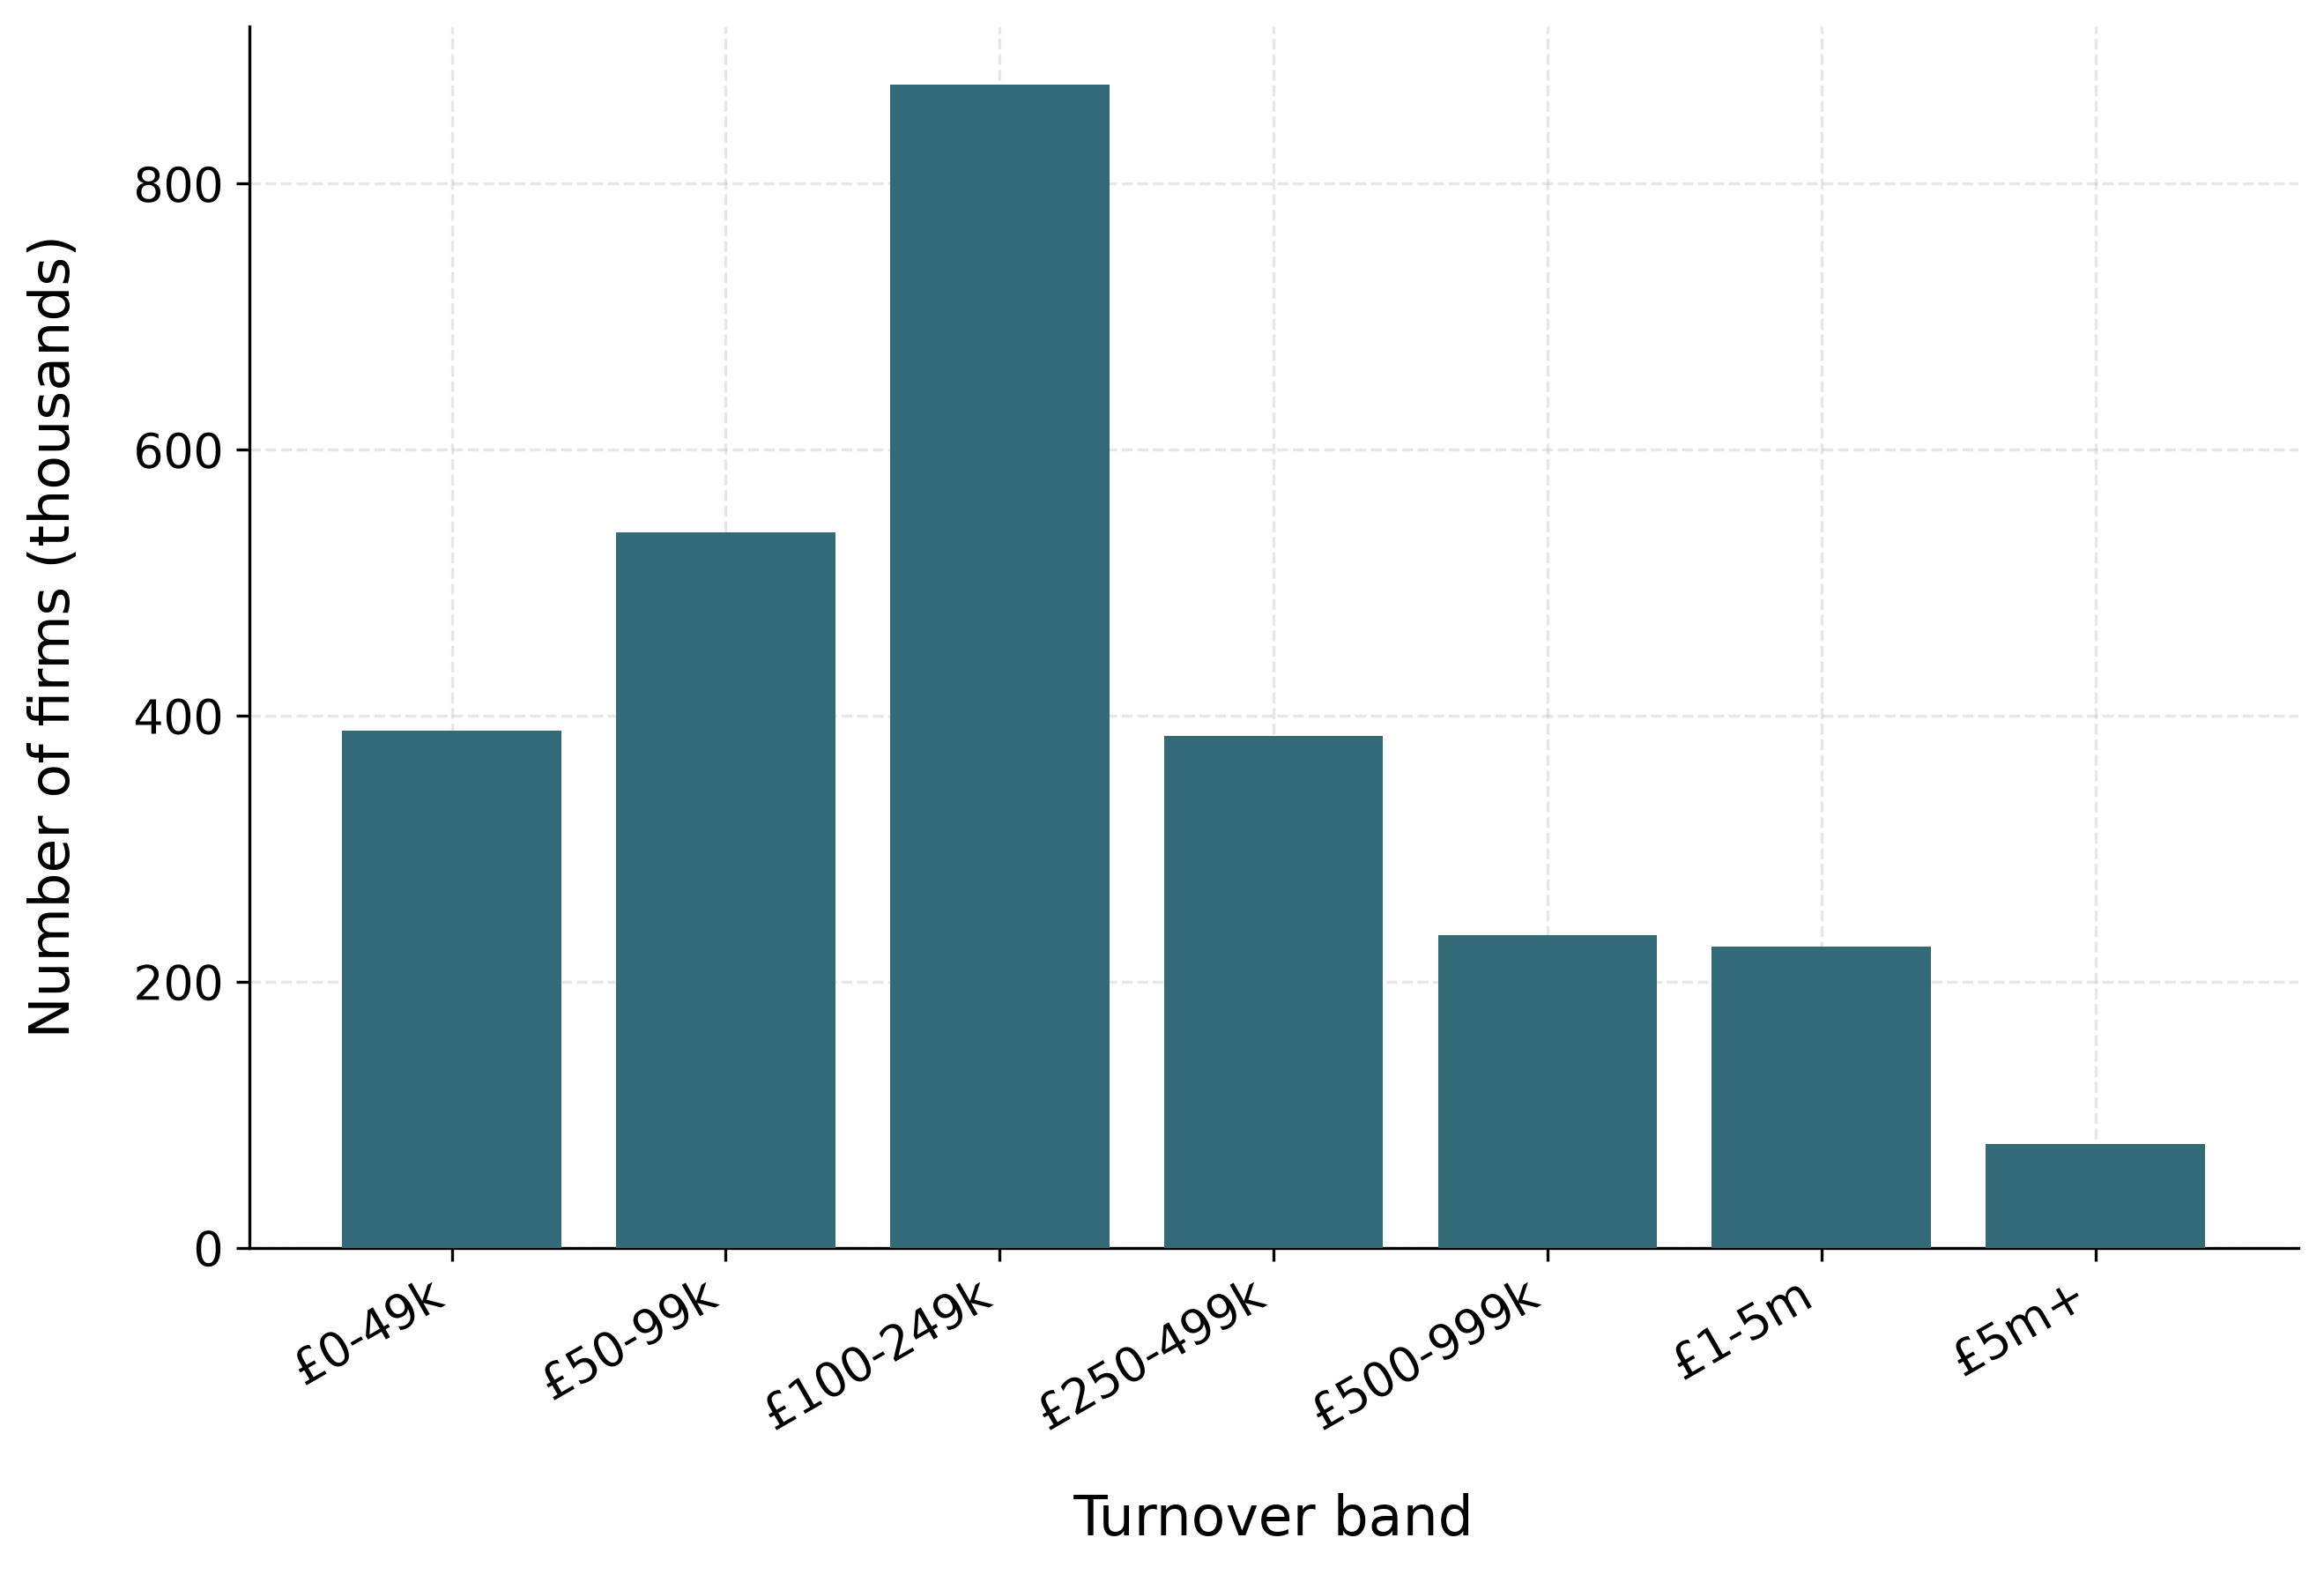
\includegraphics[width=0.48\textwidth]{figures/firms_by_turnover_band_85k.png}
}
\hfill
\subfigure[VAT-registered firms (HMRC, 2023--24)]{
    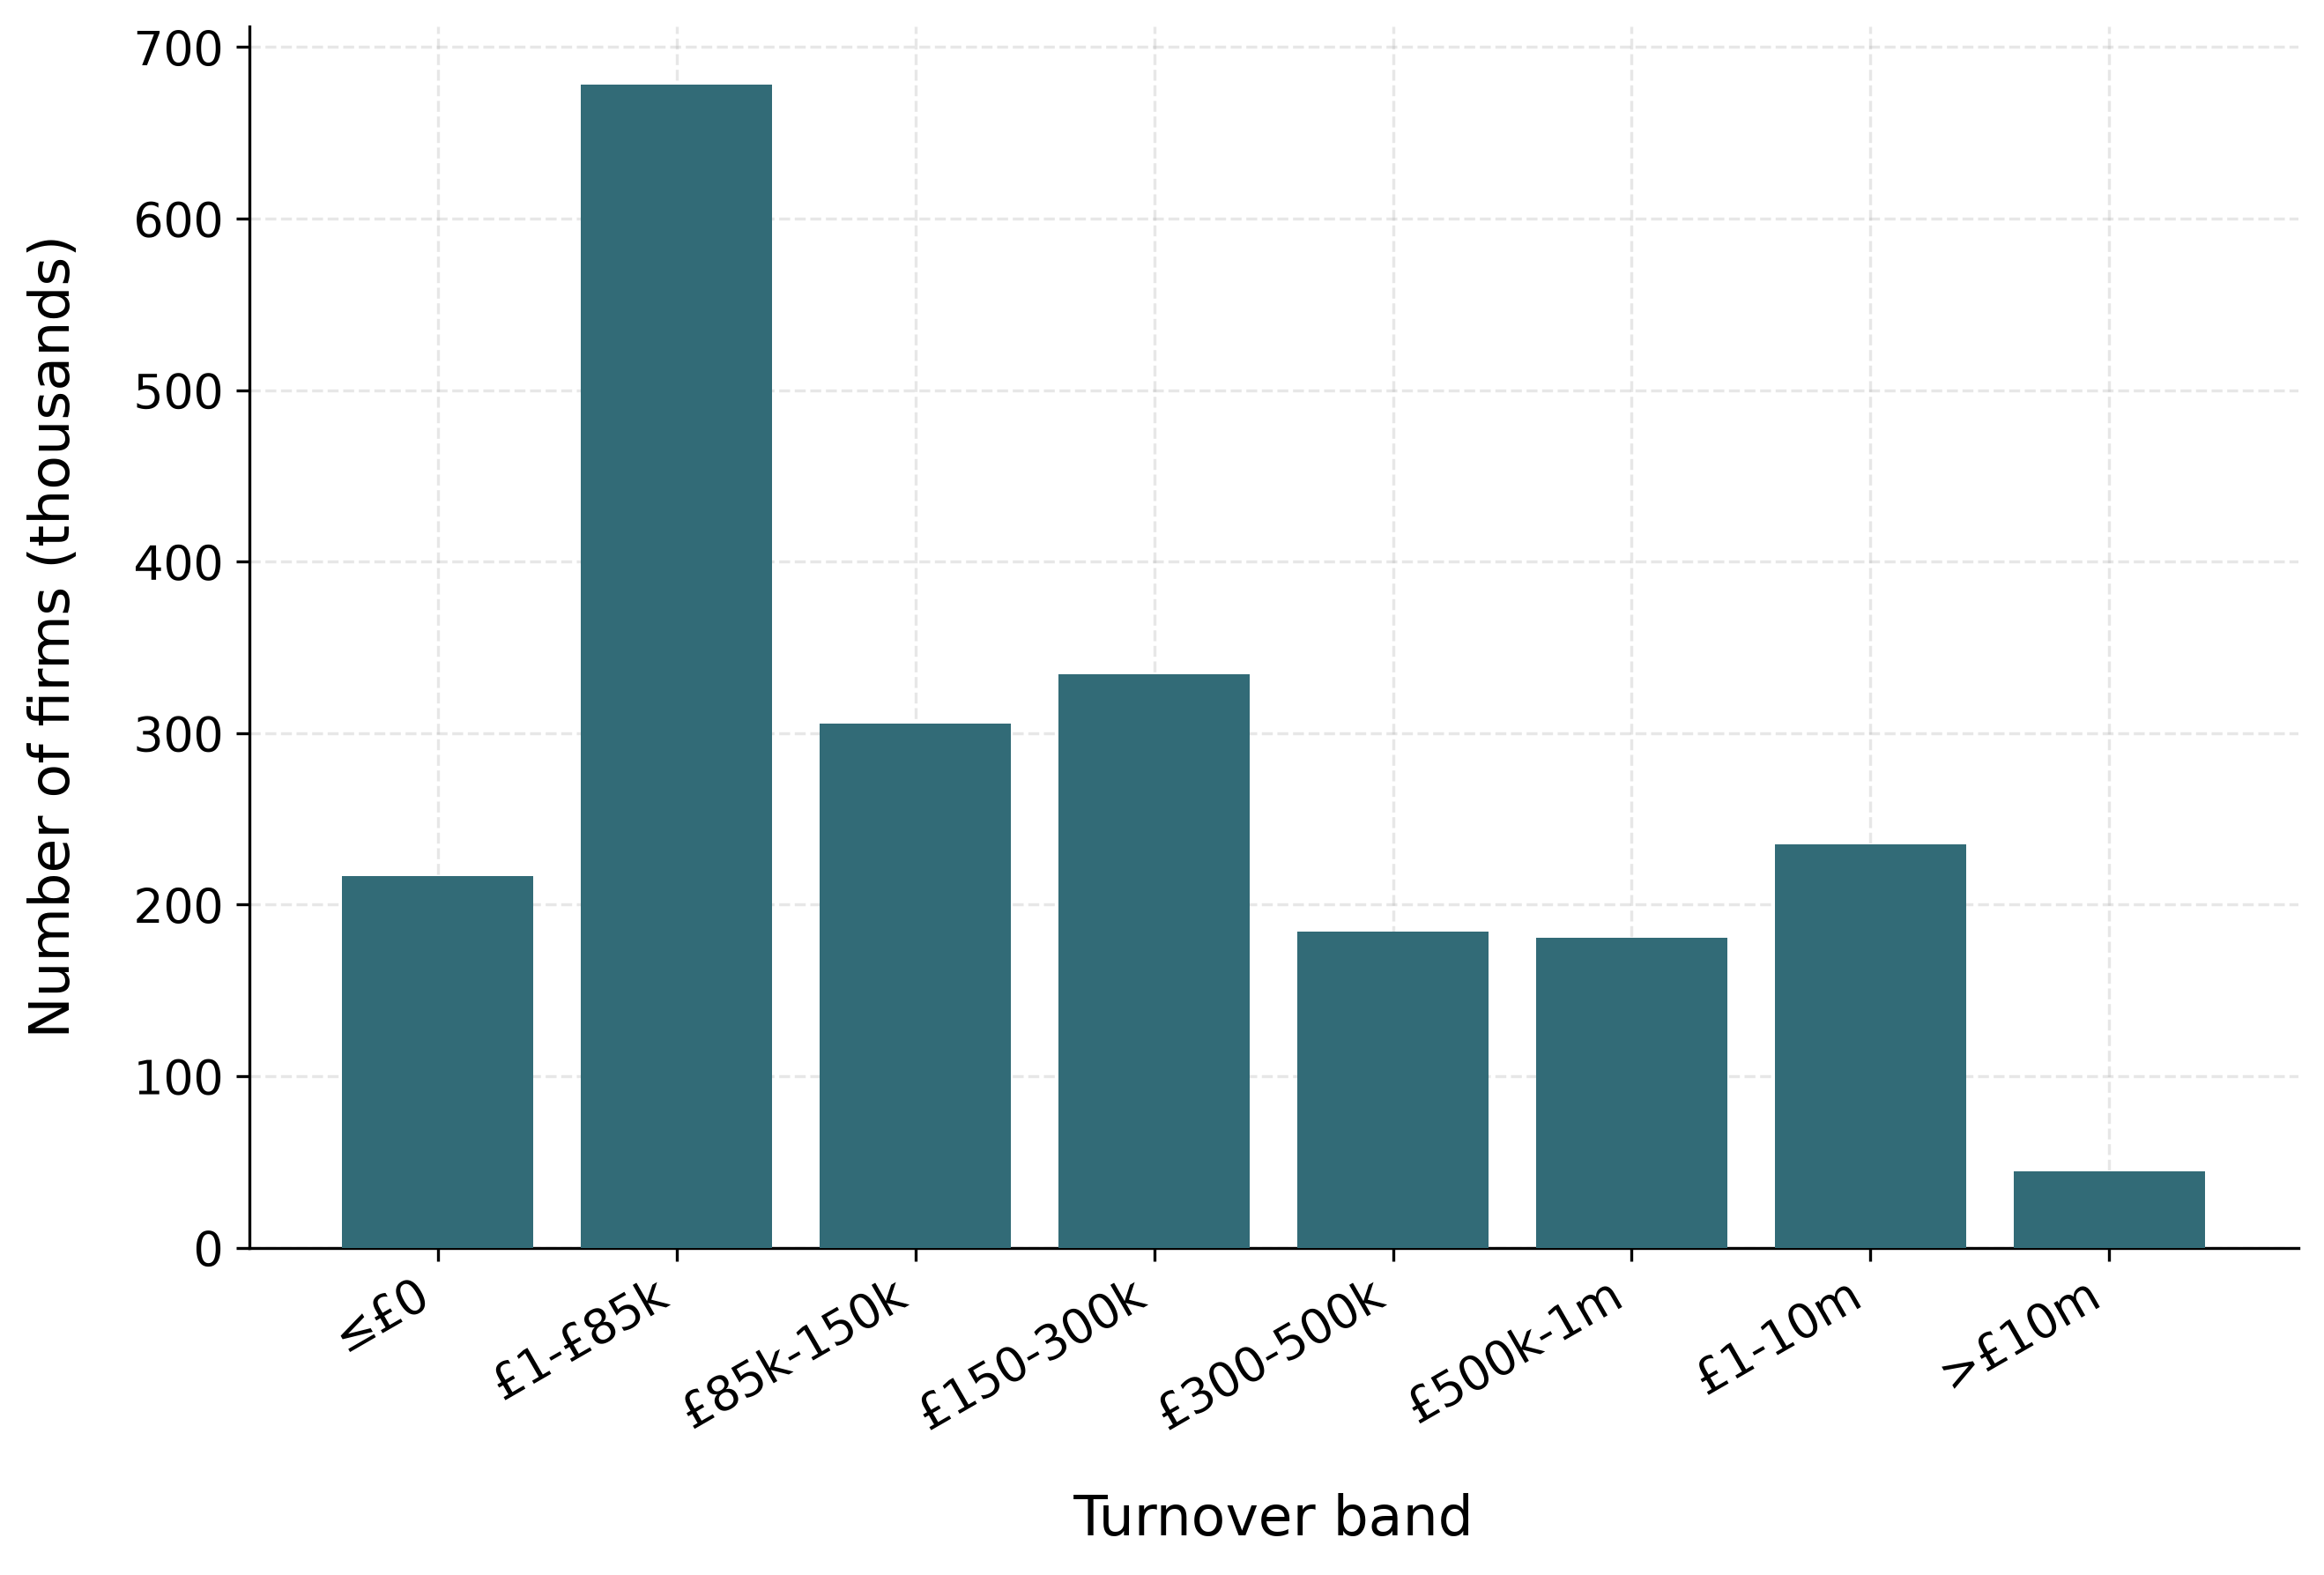
\includegraphics[width=0.48\textwidth]{figures/vat_firms_by_turnover_band_85k.png}
}
\caption{The UK firm-size distribution and VAT registration, 2023--24 (threshold
\pounds 85{,}000). Panel (a): number of businesses by turnover band in the ONS
business register, which covers businesses registered for VAT and/or PAYE
(about 2.7 million); the full business population including unregistered
businesses is roughly twice as large (DBT business population estimates).
Panel (b): number of VAT-registered firms by turnover band. Band widths are
unequal, so cross-band count comparisons should be read per \pounds1{,}000 of
turnover. Source: panel (a), ONS,
\href{https://www.ons.gov.uk/businessindustryandtrade/business/activitysizeandlocation/bulletins/ukbusinessactivitysizeandlocation/2023}{\emph{UK Business: Activity, Size and Location}}
(business counts by turnover band); panel (b), HMRC,
\href{https://www.gov.uk/government/statistics/value-added-tax-vat-annual-statistics}{\emph{Value Added Tax (VAT) Annual Statistics}}
(VAT-registered population by turnover band).}
\label{fig:dist}
\end{figure}

Firms respond to the notch by locating below the threshold. Tabulations of HMRC turnover
data show the number of firms rising towards \pounds 84{,}000 and then dropping sharply at
the \pounds 85{,}000 threshold, leaving excess mass just below it \citep{obr2023vat}.
\citet{liuetal2021} document this bunching in UK administrative firm data over
2004--05 to 2014--15, when the threshold rose from \pounds58{,}000 to
\pounds81{,}000, and \citet{liulockwoodtam2024}
find that firms slow their turnover growth as they approach the threshold. The notch
therefore distorts the size distribution and the growth decisions of firms near the margin,
which places the threshold under recurrent pressure for reform.

Reform proposals change the threshold in one of three ways: its \emph{level} (raising or lowering it), its \emph{shape} (replacing the notch with a schedule that phases the rate in over a band), or its \emph{rate} (a reduced rate for firms in a band above the threshold). The three are not equivalent. Changing the level moves the notch along the turnover axis; changing the shape or the rate alters the size of the discrete jump itself. Costing the three on a common basis is the practical difficulty this paper addresses. A change in the level can be costed by mechanical accounting, but a change in the shape of the schedule cannot be evaluated with the reduced-form bunching methods used to study the threshold, because a continuous schedule leaves no single point of excess mass to exploit. The firm-level data needed to study turnover near the threshold is, in addition, not available in open form.

In this paper I build an open, reproducible firm-level microsimulation for costing UK VAT threshold reforms on a common static basis. I construct synthetic firm microdata calibrated to published official aggregates---HMRC registered-firm counts by turnover band and by sector, net VAT liability by turnover band, and ONS business counts and employment bands---for the 2023--24 tax year, when the threshold was \pounds 85{,}000, and separately for 2024--25, when it rose to \pounds 90{,}000. Each firm's net VAT liability is the standard rate applied to its value added. The synthetic data can be released openly and regenerated under any counterfactual schedule.

On these data I do four things. First, I cost level reforms and schedule reforms---a graduated taper and a reduced-rate band---statically, by applying each counterfactual schedule mechanically to the firm distribution. Second, I characterise the notch's distortion through its \emph{dominated region}---the exact, elasticity-free range of turnover above the threshold in which no firm profits from locating---and how each reform changes it. Third, I price the level and rate reforms behaviourally: each firm re-optimises its turnover within its schedule region, conditional on an assumed turnover elasticity $e$ that the data do not identify, reported as an $e$-sensitivity range that nests the static costing exactly in its $e\to0$ limit. Fourth, I show that the synthetic data's near-threshold structure is target-inherited and cannot support bunching inference: the \pounds85{,}000 profile is calibrated to the OBR's published \pounds1{,}000-band data and the estimator reads exactly that back, a placebo without the fine targets returns zero, and the uncalibrated \pounds90{,}000 vintage shows a spurious band-edge signal.

Four findings follow. First, the static pipeline prices all the reforms on a common basis, and its anchor costing tracks the Government's published number once the deregistration convention is stated. My static costing of the April 2024 increase from \pounds 85{,}000 to \pounds 90{,}000 depends on what released firms are assumed to do: if every firm in the band deregisters, the 2025--26 cost is \pounds 323m, overshooting HMRC's published \pounds 185m \citep{hmt_spring_budget_2024} in line with the official costing's phased registration response; if the roughly 43\% voluntary-registration share that \citet{liuetal2021} document is retained, it is \pounds 184m---matching the published figure to \pounds 1m. Both conventions reproduce the official profile's narrowing and its 2028--29 sign change. Forward moves from the \pounds 90{,}000 base range from a gain of about \pounds 1{,}040m at \pounds 70{,}000 to a cost of about \pounds 1{,}450m at \pounds 120{,}000, against a base of about \pounds 200.9bn in 2025--26.

Second, the shape and rate reforms act on the notch's distortion in a way that a change in level does not. The notch creates a \emph{dominated region} of width $a = T^{*}\tau/(1-\tau) = \pounds 21{,}250$ above the threshold (\pounds 85{,}000--\pounds 106{,}250), a range of turnover in which no firm can locate without being strictly worse off than at the threshold. This region is an exact property of the schedule: under the value-added formulation of Section~\ref{sec:behavioural} its width is the same for every firm with positive value added, whatever its input share, and it requires no behavioural calibration. It also spans a populous part of the firm distribution---about 156{,}000 weighted firms in the calibrated data---so its width is an economically meaningful distortion index. Raising the threshold relocates this region without removing it. A reduced rate does \emph{not} remove it: the jump at the threshold falls (from \pounds 17{,}000 to \pounds 12{,}750 at a 15\% band), but the band reverts to the standard rate at its \pounds 105{,}000 top, introducing a second notch and a second dominated region, so the total dominated width is essentially unchanged---\pounds 21{,}562 at 15\% and \pounds 22{,}569 at 10\%, both marginally above the \pounds 21{,}250 baseline. Only the graduated taper, being continuous, removes the dominated region. On the common \pounds 85{,}000 data-year base, raising the threshold to \pounds 100{,}000 costs \pounds 753m and removes none of the dominated region; the taper removes all of it for \pounds 520m; and the 10\% and 15\% reduced rates cost \pounds 484m and \pounds 242m while splitting the dominated band in two. On the dominated-region metric the level move is the most expensive option per unit of distortion removed---a comparison that indexes the misallocation distortion only and omits the compliance-cost saving a higher threshold delivers (Section~\ref{sec:conclusion}).

Third, conditional on the assumed elasticity, intensive-margin responses barely move these costings. A pure level rise has \emph{exactly} zero intensive-margin revenue offset at every $e$: released firms leave the VAT base, so their expansion is untaxed, and no other firm's effective rate changes---a result the simulator verifies to \pounds0.1m. For the reduced-rate bands the offset is second order: at $e=0.17$ the 10\% band's cost falls from \pounds 484m to \pounds 475m and the 15\% band's from \pounds 242m to \pounds 235m, under 6\% even at $e=0.32$. I do not report a behavioural cost for the graduated taper: its rate varies continuously with turnover, so its marginal-rate channel is outside the flat-rate machinery, and only its static cost and dominated-region removal are reported. The sweep values $e \in \{0.05, 0.17, 0.32\}$ are assumptions: the lower end has an external anchor \citep{klevenwaseem2013}, and the published UK VAT-base estimates of \citet{liuetal2021} fall between it and the midpoint. The consequence of these results runs opposite to the usual worry: the static costings are robust to the intensive margin, and the behavioural uncertainty that matters---registration and location choice at the notch---is exactly the margin the synthetic data cannot identify.

Fourth, the open data carry a transparency lesson about bunching: every sub-band feature of band-calibrated synthetic data is exactly what its targets put there, and this paper demonstrates the point in three directions. The 2023--24 population's near-threshold density is calibrated to the OBR's published \pounds1{,}000-band profile \citep{obr2023vat}, so it reproduces the administratively observed bunching shape---and the estimator reads that shape back as excess mass ($E=7{,}933$), which is target inheritance, not behaviour. A placebo that regenerates the population \emph{without} the fine targets returns $E=0$: remove the targets and the ``bunching'' vanishes. And the 2024--25 vintage, for which no fine bands are published, shows what the trap looks like from the other side: the coarse \pounds90{,}000 band edge alone produces an excess-bunching statistic within 10\% of the administrative estimate of \citet{liuetal2021}---a coincidence of band geometry, four-fold unstable across estimator specifications, with no behaviour behind it. An earlier draft of this paper reported ``reproducing'' the administrative step when a liability mis-scaling in the generator manufactured it; the correction removed it, and the OBR targets now supply the shape from published data instead. The lesson is symmetric and general: synthetic bunching is not evidence of behaviour, its absence is not evidence of no behaviour, and any sub-band feature of calibrated data should be traced to its targets before it is read as economics. The behavioural evidence on UK VAT bunching remains \citeauthor{liuetal2021}'s administrative estimate.

\subsection*{Related literature}

The paper draws on four strands of work. The first is the methodology of bunching and notches \citep{chettyetal2011,saez2010,klevenwaseem2013,kleven2016,best2015}, which provides the analytic notion of a dominated region; I use the dominated region to characterise a distortion that leaves no single point of excess mass to exploit.

The second is the empirical literature on VAT registration thresholds \citep{liuetal2021,liulockwoodtam2024,onji2009,harju2019,asatryanpeichl2017,nandiwarwick2020,waseem2024}. \citet{liuetal2021} is closest: it estimates bunching at the UK notch on administrative data over 2004--2014 and documents voluntary registration; I take its estimates as the established behavioural facts and cost shape and rate reforms statically on a common basis, which that literature does not do. The international evidence \citep{harju2019,onji2009,asatryanpeichl2017,nandiwarwick2020} notes that bunching at a VAT threshold can reflect compliance costs, firm-splitting, or reporting rather than real turnover responses.

The third strand questions whether bunching identifies a structural elasticity at all: \citet{blomquistetal2021} show that the elasticity is not non-parametrically identified from bunching at a kink or a notch without strong functional-form assumptions, and \citet{bertanhaetal2023} develop the notch case. This literature motivates my refusal to read an elasticity off the synthetic data: even setting aside the placebo evidence that any synthetic step is mechanical, the mapping from excess mass to an elasticity requires assumptions I am unwilling to impose. The fourth strand is the structural literature on size-based thresholds \citep{garicano2016,gourioroys2014}, which identifies policy-invariant primitives at the French 50-employee threshold and computes welfare from them; the present paper makes no such structural claim.

This paper makes three contributions. First, it provides an open, reproducible firm-level microsimulation for costing UK VAT threshold reforms, where the existing firm-level evidence rests on restricted administrative data; the released pipeline regenerates every number in the paper from public inputs. Second, it characterises the notch's distortion through its exact dominated region and costs two schedule reforms---a graduated taper and a reduced-rate band---on the same static basis as level reforms. Third, it demonstrates, by construction and by correction, that band-calibrated synthetic data carry no sub-band behavioural information beyond their targets: the paper documents how its own earlier build manufactured a plausible-looking density step, how the correction removed it, how calibrating to the OBR's published fine bands restores the administrative shape as an explicit target, and how the same band-edge mechanism manufactures a spurious signal where no fine targets exist. Identifying the turnover elasticity from administrative micro-data, a welfare accounting, revenue-neutral designs, and an explicit model of voluntary registration are left for future work.

The remainder of the paper proceeds as follows. Section~\ref{sec:background} describes the institutional background of the UK VAT threshold. Section~\ref{sec:data} sets out the synthetic firm microdata and its calibration to official aggregates. Section~\ref{sec:static} sets out the static costing of threshold changes and the schedule reforms. Section~\ref{sec:bunching} shows that the synthetic data contain no usable bunching signal and validates the estimator's power on injected signals. Section~\ref{sec:model} develops the notch and its exact dominated region, and shows how each reform changes it. Section~\ref{sec:behavioural} prices the reforms behaviourally, conditional on an assumed elasticity, and derives the level-rise invariance. Section~\ref{sec:conclusion} concludes.
